% Options for packages loaded elsewhere
\PassOptionsToPackage{unicode}{hyperref}
\PassOptionsToPackage{hyphens}{url}
%
\documentclass[
  ignorenonframetext,
]{beamer}
\usepackage{pgfpages}
\setbeamertemplate{caption}[numbered]
\setbeamertemplate{caption label separator}{: }
\setbeamercolor{caption name}{fg=normal text.fg}
\beamertemplatenavigationsymbolsempty
% Prevent slide breaks in the middle of a paragraph
\widowpenalties 1 10000
\raggedbottom
\setbeamertemplate{part page}{
  \centering
  \begin{beamercolorbox}[sep=16pt,center]{part title}
    \usebeamerfont{part title}\insertpart\par
  \end{beamercolorbox}
}
\setbeamertemplate{section page}{
  \centering
  \begin{beamercolorbox}[sep=12pt,center]{part title}
    \usebeamerfont{section title}\insertsection\par
  \end{beamercolorbox}
}
\setbeamertemplate{subsection page}{
  \centering
  \begin{beamercolorbox}[sep=8pt,center]{part title}
    \usebeamerfont{subsection title}\insertsubsection\par
  \end{beamercolorbox}
}
\AtBeginPart{
  \frame{\partpage}
}
\AtBeginSection{
  \ifbibliography
  \else
    \frame{\sectionpage}
  \fi
}
\AtBeginSubsection{
  \frame{\subsectionpage}
}
\usepackage{amsmath,amssymb}
\usepackage{iftex}
\ifPDFTeX
  \usepackage[T1]{fontenc}
  \usepackage[utf8]{inputenc}
  \usepackage{textcomp} % provide euro and other symbols
\else % if luatex or xetex
  \usepackage{unicode-math} % this also loads fontspec
  \defaultfontfeatures{Scale=MatchLowercase}
  \defaultfontfeatures[\rmfamily]{Ligatures=TeX,Scale=1}
\fi
\usepackage{lmodern}
\ifPDFTeX\else
  % xetex/luatex font selection
\fi
% Use upquote if available, for straight quotes in verbatim environments
\IfFileExists{upquote.sty}{\usepackage{upquote}}{}
\IfFileExists{microtype.sty}{% use microtype if available
  \usepackage[]{microtype}
  \UseMicrotypeSet[protrusion]{basicmath} % disable protrusion for tt fonts
}{}
\makeatletter
\@ifundefined{KOMAClassName}{% if non-KOMA class
  \IfFileExists{parskip.sty}{%
    \usepackage{parskip}
  }{% else
    \setlength{\parindent}{0pt}
    \setlength{\parskip}{6pt plus 2pt minus 1pt}}
}{% if KOMA class
  \KOMAoptions{parskip=half}}
\makeatother
\usepackage{xcolor}
\newif\ifbibliography
\usepackage{color}
\usepackage{fancyvrb}
\newcommand{\VerbBar}{|}
\newcommand{\VERB}{\Verb[commandchars=\\\{\}]}
\DefineVerbatimEnvironment{Highlighting}{Verbatim}{commandchars=\\\{\}}
% Add ',fontsize=\small' for more characters per line
\usepackage{framed}
\definecolor{shadecolor}{RGB}{248,248,248}
\newenvironment{Shaded}{\begin{snugshade}}{\end{snugshade}}
\newcommand{\AlertTok}[1]{\textcolor[rgb]{0.94,0.16,0.16}{#1}}
\newcommand{\AnnotationTok}[1]{\textcolor[rgb]{0.56,0.35,0.01}{\textbf{\textit{#1}}}}
\newcommand{\AttributeTok}[1]{\textcolor[rgb]{0.13,0.29,0.53}{#1}}
\newcommand{\BaseNTok}[1]{\textcolor[rgb]{0.00,0.00,0.81}{#1}}
\newcommand{\BuiltInTok}[1]{#1}
\newcommand{\CharTok}[1]{\textcolor[rgb]{0.31,0.60,0.02}{#1}}
\newcommand{\CommentTok}[1]{\textcolor[rgb]{0.56,0.35,0.01}{\textit{#1}}}
\newcommand{\CommentVarTok}[1]{\textcolor[rgb]{0.56,0.35,0.01}{\textbf{\textit{#1}}}}
\newcommand{\ConstantTok}[1]{\textcolor[rgb]{0.56,0.35,0.01}{#1}}
\newcommand{\ControlFlowTok}[1]{\textcolor[rgb]{0.13,0.29,0.53}{\textbf{#1}}}
\newcommand{\DataTypeTok}[1]{\textcolor[rgb]{0.13,0.29,0.53}{#1}}
\newcommand{\DecValTok}[1]{\textcolor[rgb]{0.00,0.00,0.81}{#1}}
\newcommand{\DocumentationTok}[1]{\textcolor[rgb]{0.56,0.35,0.01}{\textbf{\textit{#1}}}}
\newcommand{\ErrorTok}[1]{\textcolor[rgb]{0.64,0.00,0.00}{\textbf{#1}}}
\newcommand{\ExtensionTok}[1]{#1}
\newcommand{\FloatTok}[1]{\textcolor[rgb]{0.00,0.00,0.81}{#1}}
\newcommand{\FunctionTok}[1]{\textcolor[rgb]{0.13,0.29,0.53}{\textbf{#1}}}
\newcommand{\ImportTok}[1]{#1}
\newcommand{\InformationTok}[1]{\textcolor[rgb]{0.56,0.35,0.01}{\textbf{\textit{#1}}}}
\newcommand{\KeywordTok}[1]{\textcolor[rgb]{0.13,0.29,0.53}{\textbf{#1}}}
\newcommand{\NormalTok}[1]{#1}
\newcommand{\OperatorTok}[1]{\textcolor[rgb]{0.81,0.36,0.00}{\textbf{#1}}}
\newcommand{\OtherTok}[1]{\textcolor[rgb]{0.56,0.35,0.01}{#1}}
\newcommand{\PreprocessorTok}[1]{\textcolor[rgb]{0.56,0.35,0.01}{\textit{#1}}}
\newcommand{\RegionMarkerTok}[1]{#1}
\newcommand{\SpecialCharTok}[1]{\textcolor[rgb]{0.81,0.36,0.00}{\textbf{#1}}}
\newcommand{\SpecialStringTok}[1]{\textcolor[rgb]{0.31,0.60,0.02}{#1}}
\newcommand{\StringTok}[1]{\textcolor[rgb]{0.31,0.60,0.02}{#1}}
\newcommand{\VariableTok}[1]{\textcolor[rgb]{0.00,0.00,0.00}{#1}}
\newcommand{\VerbatimStringTok}[1]{\textcolor[rgb]{0.31,0.60,0.02}{#1}}
\newcommand{\WarningTok}[1]{\textcolor[rgb]{0.56,0.35,0.01}{\textbf{\textit{#1}}}}
\usepackage{graphicx}
\makeatletter
\def\maxwidth{\ifdim\Gin@nat@width>\linewidth\linewidth\else\Gin@nat@width\fi}
\def\maxheight{\ifdim\Gin@nat@height>\textheight\textheight\else\Gin@nat@height\fi}
\makeatother
% Scale images if necessary, so that they will not overflow the page
% margins by default, and it is still possible to overwrite the defaults
% using explicit options in \includegraphics[width, height, ...]{}
\setkeys{Gin}{width=\maxwidth,height=\maxheight,keepaspectratio}
% Set default figure placement to htbp
\makeatletter
\def\fps@figure{htbp}
\makeatother
\setlength{\emergencystretch}{3em} % prevent overfull lines
\providecommand{\tightlist}{%
  \setlength{\itemsep}{0pt}\setlength{\parskip}{0pt}}
\setcounter{secnumdepth}{-\maxdimen} % remove section numbering
\usepackage[utf8]{inputenc}
\usepackage{longtable}
\usepackage{here}
\ifLuaTeX
  \usepackage{selnolig}  % disable illegal ligatures
\fi
\IfFileExists{bookmark.sty}{\usepackage{bookmark}}{\usepackage{hyperref}}
\IfFileExists{xurl.sty}{\usepackage{xurl}}{} % add URL line breaks if available
\urlstyle{same}
\hypersetup{
  pdftitle={Grupos de Experimentos},
  pdfauthor={Renata Alcarde Sermarini},
  hidelinks,
  pdfcreator={LaTeX via pandoc}}

\title{Grupos de Experimentos}
\author{Renata Alcarde Sermarini}
\date{novembro de 2020}

\begin{document}
\frame{\titlepage}

\begin{frame}{Exemplo (Barbin, 1994)}
\protect\hypertarget{exemplo-barbin-1994}{}
Os dados que se seguem referem-se a alturas (em metros, médias de 25
plantas/parcela) de plantas Eucaliptus grandis, com 7 anos de idade (em
1980) de três ensaios em blocos ao acaso, sob 6 tratamentos (progênies).

\begin{center}
\begin{tabular}{lccccr} 
\multicolumn{6}{l}{Tabela 1: Ensaio em Araraquara}\\ \hline
 & \multicolumn{4}{c}{Blocos} & \\ \cline{2-5}
Tratamentos &   I & II &    III &   IV  & Totais \\ \hline
T1 &    20,3 &  19,6 &  23,5 &  19,1 &  82,5\\
T2 &    21,7 &  19,3 &  16,7 &  18,5 &  76,2\\
T3 &    22,0 &  24,9 &  24,4 &  20,8 &  92,1\\
T4 &    20,8 &  23,0 &  21,3 &  24,9 &  90,0\\
T5 &    21,5 &  22,3 &  22,1 &  21,9 &  87,8\\
T6 &    19,6 &  17,7 &  18,7 &  22,0 &  78,0\\ \hline
Totais &    125,9 & 126,8 & 126,7 & 127,2   506,6\\ \hline
\multicolumn{6}{l}{Fonte: Instituto Florestal – Tupi, SP}\\
\end{tabular}
\end{center}
\end{frame}

\begin{frame}{Exemplo (Barbin, 1994)}
\protect\hypertarget{exemplo-barbin-1994-1}{}
\begin{center}
\begin{tabular}{lccccr} 
\multicolumn{6}{l}{Tabela 2: Ensaio em Bento Quirino}\\ \hline
 & \multicolumn{4}{c}{Blocos} & \\ \cline{2-5}
Tratamentos &   I & II &    III &   IV  & Totais \\ \hline
T1 &    10,2 &  11,7 &  9,1 &   8,1 & 39,1 \\
T2 &    16,1 &  10,8 &  10,9 &  10,3 &  48,1 \\ 
T3 &    17,7 &  13,1 &  14,2 &  11,0 &  56,0\\
T4 &    13,5 &  14,4 &  11,2 &  12,8 &  51,9\\
T5 &    20,5 &  12,5 &  11,3 &  12,2 &  56,5\\
T6 &    12,0 &  13,0 &  12,3 &  10,6 &  47,9\\ \hline
Totais  &   90,0 &  75,5 &  69,0 &  65,0 &  299,5 \\ \hline
\multicolumn{6}{l}{Fonte: Instituto Florestal – Tupi, SP}\\
\end{tabular}
\end{center}

T1: Pretoria (Procedente da África do Sul), T2: 637 (Progênie de Rio
Claro), T3: 2093 (Progênie de Rio Claro), T4: 2094 (Progênie de Rio
Claro), T5: 9559 (Procedente da Austrália) e T6: 9575 (Procedente da
Austrália).
\end{frame}

\begin{frame}{Exemplo (Barbin, 1994)}
\protect\hypertarget{exemplo-barbin-1994-2}{}
\begin{center}
\begin{tabular}{lccccr} 
\multicolumn{6}{l}{Tabela 3: Ensaio em Mogi-Guaçu}\\ \hline
 & \multicolumn{4}{c}{Blocos} & \\ \cline{2-5}
Tratamentos &   I & II &    III &   IV  & Totais \\ \hline
T1 &    22,7 &  21,4 &  22,9 &  22,0 &  89,0\\
T2 &    22,6 &  21,4 &  20,7 &  20,8 &  85,5\\
T3 &    21,4 &  21,7 &  22,5 &  19,4 &  85,0\\
T4 &    25,0 &  23,6 &  23,3 &  24,8 &  96,7\\
T5 &    26,4 &  26,4 &  28,0 &  27,3 &  108,1\\
T6 &    20,6 &  23,5 &  19,4 &  21,9 &  85,4\\
Totais &    138,7 & 138,0 & 136,8 & 136,2 & 549,7\\ \hline
\multicolumn{6}{l}{Fonte: Instituto Florestal – Tupi, SP}\\
\end{tabular}
\end{center}

T1: Pretoria (Procedente da África do Sul), T2: 637 (Progênie de Rio
Claro), T3: 2093 (Progênie de Rio Claro), T4: 2094 (Progênie de Rio
Claro), T5: 9559 (Procedente da Austrália) e T6: 9575 (Procedente da
Austrália).

Observação: Os dados foram cedidos pelo Engenheiro Agrônomo Luiz Carlos
Costa Coelho do Horto Florestal de Tupi, SP.
\end{frame}

\begin{frame}[fragile]{Entrada dos dados}
\protect\hypertarget{entrada-dos-dados}{}
\begin{Shaded}
\begin{Highlighting}[]
\NormalTok{dados}\OtherTok{\textless{}{-}} \FunctionTok{read.csv2}\NormalTok{(}\StringTok{"eucalipto.csv"}\NormalTok{)}
\FunctionTok{str}\NormalTok{(dados)}
\end{Highlighting}
\end{Shaded}

\begin{verbatim}
## 'data.frame':    72 obs. of  4 variables:
##  $ Local : chr  "L1" "L1" "L1" "L1" ...
##  $ Bloco : chr  "B1" "B1" "B1" "B1" ...
##  $ Trat  : chr  "T1" "T2" "T3" "T4" ...
##  $ altura: num  20.3 21.7 22 20.8 21.5 19.6 19.6 19.3 24.9 23 ...
\end{verbatim}
\end{frame}

\begin{frame}[fragile]{Análise exploratória}
\protect\hypertarget{anuxe1lise-exploratuxf3ria}{}
\begin{Shaded}
\begin{Highlighting}[]
\FunctionTok{ggplot}\NormalTok{(dados,}
       \FunctionTok{aes}\NormalTok{(}\AttributeTok{x =}\NormalTok{ Trat,}
           \AttributeTok{y =}\NormalTok{ altura,}
           \AttributeTok{color =}\NormalTok{ Trat)) }\SpecialCharTok{+} 
  \FunctionTok{geom\_point}\NormalTok{() }\SpecialCharTok{+}
  \FunctionTok{facet\_wrap}\NormalTok{(}\SpecialCharTok{\textasciitilde{}}\NormalTok{Local) }\SpecialCharTok{+}
  \FunctionTok{xlab}\NormalTok{(}\StringTok{"Tratamentos"}\NormalTok{) }\SpecialCharTok{+}
  \FunctionTok{ylab}\NormalTok{(}\StringTok{"altura (m)"}\NormalTok{) }\SpecialCharTok{+}
  \FunctionTok{theme\_bw}\NormalTok{() }\SpecialCharTok{+}
  \FunctionTok{theme}\NormalTok{(}\AttributeTok{legend.position =} \StringTok{"bottom"}\NormalTok{,}
        \AttributeTok{legend.direction =} \StringTok{"horizontal"}\NormalTok{,}
        \AttributeTok{legend.title =} \FunctionTok{element\_blank}\NormalTok{())}
\end{Highlighting}
\end{Shaded}
\end{frame}

\begin{frame}{Análise exploratória}
\protect\hypertarget{anuxe1lise-exploratuxf3ria-1}{}
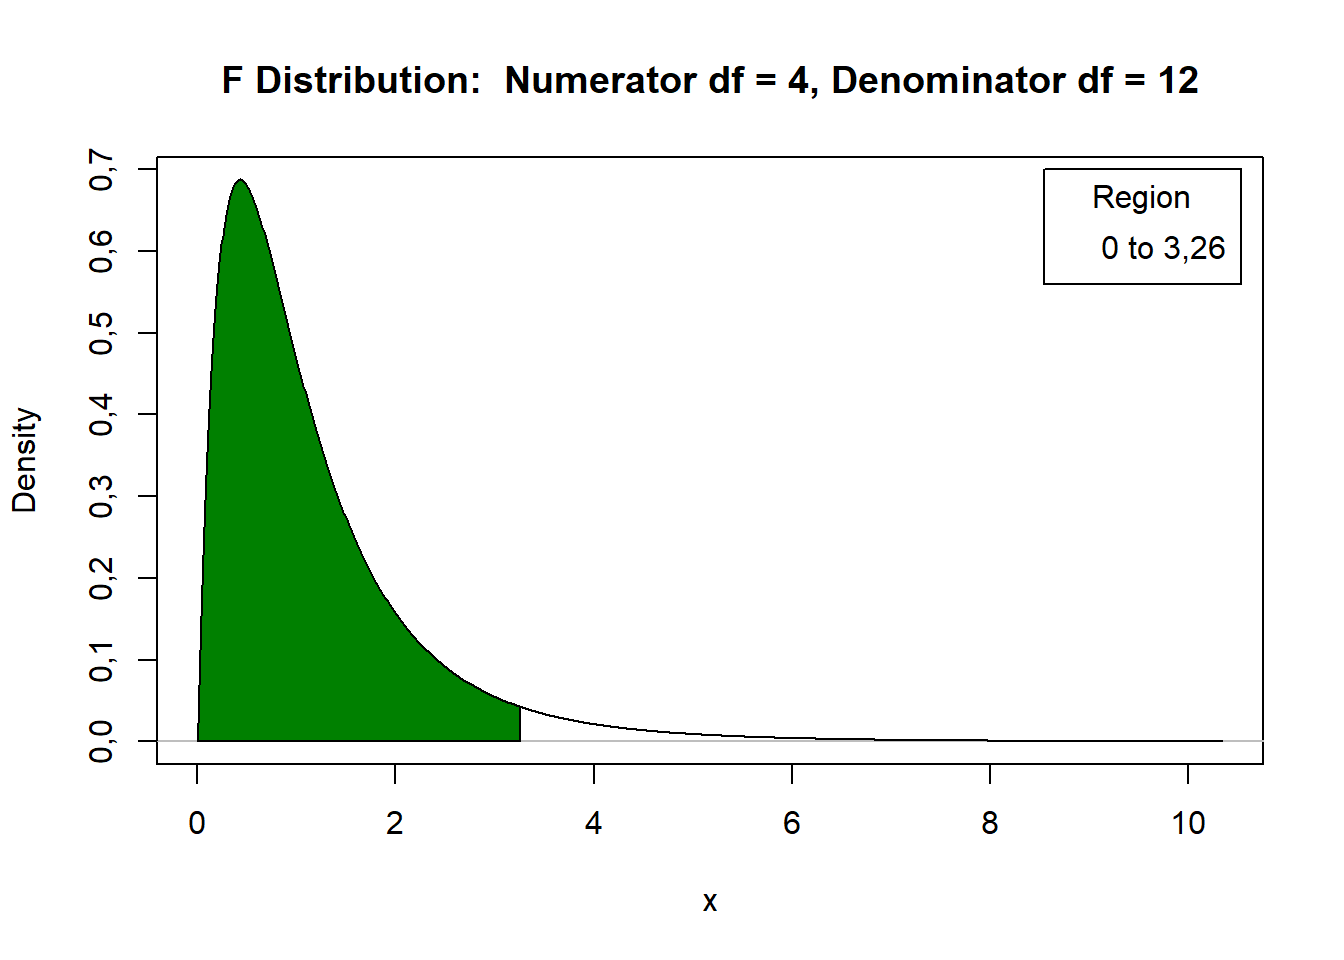
\includegraphics{aula12_GruposdeExp_files/figure-beamer/unnamed-chunk-4-1.pdf}
\end{frame}

\begin{frame}{Trabalhando com grupos de Experimentos}
\protect\hypertarget{trabalhando-com-grupos-de-experimentos}{}
\begin{itemize}
\tightlist
\item
  Os experimentos são instalados em locais distintos ou em tempos
  distintos (repetição do experimento);
\item
  De modo geral, em casos completos e balanceados, os mesmos tratamentos
  são avaliados em cada um dos experimentos, seguindo o mesmo
  delineamento e o mesmo número de repetições.
\end{itemize}

\textbf{Quando podemos agrupar os dados para a análise?}

Em caso de homogeneidade de variâncias!

\emph{Vantagens}:

\begin{itemize}
\item
  Avaliar o efeito da interação Local\#Tratamento (ou
  Repetição\#Tratamento - \textbf{Cuidado!})
\item
  Maior número de graus de liberdade do resíduo.
\end{itemize}
\end{frame}

\begin{frame}{Procedimento}
\protect\hypertarget{procedimento}{}
\begin{itemize}
\tightlist
\item
  Realizar a análise de variância individual;
\item
  Obter o coeficiente de variação;
\item
  Avaliar os efeitos de interesse (efeitos de interação e efeitos
  principais).
\end{itemize}
\end{frame}

\begin{frame}[fragile]{ANOVA Local 1: Araraquara}
\protect\hypertarget{anova-local-1-araraquara}{}
\(H_0: \mu_1 = \mu_2 = \ldots = \mu_6\) \emph{vs} \(H_1\): pelo menos
duas médias diferem entre si

\begin{Shaded}
\begin{Highlighting}[]
\NormalTok{mod.l1}\OtherTok{\textless{}{-}} \FunctionTok{aov}\NormalTok{(altura }\SpecialCharTok{\textasciitilde{}}\NormalTok{ Bloco }\SpecialCharTok{+}\NormalTok{ Trat, }
             \AttributeTok{data=}\NormalTok{dados, }
             \AttributeTok{subset=}\FunctionTok{c}\NormalTok{(Local}\SpecialCharTok{==}\StringTok{"L1"}\NormalTok{))}
\CommentTok{\# shapiro.test(rstandard(mod.l1))}
\CommentTok{\# bptest(mod.l1)}
\FunctionTok{anova}\NormalTok{(mod.l1)}
\end{Highlighting}
\end{Shaded}
\end{frame}

\begin{frame}[fragile]{ANOVA Local 1: Araraquara}
\protect\hypertarget{anova-local-1-araraquara-1}{}
\(H_0: \mu_1 = \mu_2 = \ldots = \mu_6\) \emph{vs} \(H_1\): pelo menos
duas médias diferem entre si

\begin{verbatim}
## Analysis of Variance Table
## 
## Response: altura
##           Df Sum Sq Mean Sq F value  Pr(>F)  
## Bloco      3  0.148  0.0494  0.0131 0.99786  
## Trat       5 53.503 10.7007  2.8285 0.05405 .
## Residuals 15 56.747  3.7831                  
## ---
## Signif. codes:  0 '***' 0.001 '**' 0.01 '*' 0.05 '.' 0.1 ' ' 1
\end{verbatim}

Ao nível de 5\% de significância, não há evidências para rejeitarmos
\(H_0\). Logo, não há efeito significativo de progênie quando avaliado
em Araraquara.
\end{frame}

\begin{frame}[fragile]{ANOVA Local 2: Bento Quirino}
\protect\hypertarget{anova-local-2-bento-quirino}{}
\(H_0: \mu_1 = \mu_2 = \ldots = \mu_6\) \emph{vs} \(H_1\): pelo menos
duas médias diferem entre si

\begin{Shaded}
\begin{Highlighting}[]
\NormalTok{mod.l2}\OtherTok{\textless{}{-}} \FunctionTok{aov}\NormalTok{(altura }\SpecialCharTok{\textasciitilde{}}\NormalTok{ Bloco }\SpecialCharTok{+}\NormalTok{ Trat, }
             \AttributeTok{data=}\NormalTok{dados,}
             \AttributeTok{subset=}\FunctionTok{c}\NormalTok{(Local}\SpecialCharTok{==}\StringTok{"L2"}\NormalTok{))}
\CommentTok{\# shapiro.test(rstandard(mod.l2))}
\CommentTok{\# bptest(mod.l2)}
\FunctionTok{anova}\NormalTok{(mod.l2)}
\end{Highlighting}
\end{Shaded}
\end{frame}

\begin{frame}[fragile]{ANOVA Local 2: Bento Quirino}
\protect\hypertarget{anova-local-2-bento-quirino-1}{}
\(H_0: \mu_{T1} = \mu_{T2} = \ldots = \mu_{T6}\) \emph{vs} \(H_1\): pelo
menos duas médias diferem entre si

\begin{verbatim}
## Analysis of Variance Table
## 
## Response: altura
##           Df Sum Sq Mean Sq F value  Pr(>F)  
## Bloco      3 60.198  20.066  5.3424 0.01053 *
## Trat       5 52.162  10.432  2.7776 0.05710 .
## Residuals 15 56.340   3.756                  
## ---
## Signif. codes:  0 '***' 0.001 '**' 0.01 '*' 0.05 '.' 0.1 ' ' 1
\end{verbatim}

Ao nível de 5\% de significância, não há evidências para rejeitarmos
\(H_0\). Logo, não há efeito significativo de progênie quando avaliado
em Bento Quirino.
\end{frame}

\begin{frame}[fragile]{ANOVA Local 3: Mogi-Guaçu}
\protect\hypertarget{anova-local-3-mogi-guauxe7u}{}
\(H_0: \mu_{T1} = \mu_{T2} = \ldots = \mu_{T6}\) \emph{vs} \(H_1\): pelo
menos duas médias diferem entre si

\begin{Shaded}
\begin{Highlighting}[]
\NormalTok{mod.l3}\OtherTok{\textless{}{-}} \FunctionTok{aov}\NormalTok{(altura }\SpecialCharTok{\textasciitilde{}}\NormalTok{ Bloco }\SpecialCharTok{+}\NormalTok{ Trat, }
             \AttributeTok{data=}\NormalTok{dados, }
             \AttributeTok{subset=}\FunctionTok{c}\NormalTok{(Local}\SpecialCharTok{==}\StringTok{"L3"}\NormalTok{))}
\CommentTok{\# shapiro.test(rstandard(mod.l3))}
\CommentTok{\# bptest(mod.l3)}
\FunctionTok{anova}\NormalTok{(mod.l3)}
\end{Highlighting}
\end{Shaded}
\end{frame}

\begin{frame}[fragile]{ANOVA Local 3: Mogi-Guaçu}
\protect\hypertarget{anova-local-3-mogi-guauxe7u-1}{}
\(H_0: \mu_{T1} = \mu_{T2} = \ldots = \mu_{T6}\) \emph{vs} \(H_1\): pelo
menos duas médias diferem entre si

\begin{verbatim}
## Analysis of Variance Table
## 
## Response: altura
##           Df  Sum Sq Mean Sq F value    Pr(>F)    
## Bloco      3   0.641  0.2138  0.1489    0.9288    
## Trat       5 106.057 21.2114 14.7772 2.446e-05 ***
## Residuals 15  21.531  1.4354                      
## ---
## Signif. codes:  0 '***' 0.001 '**' 0.01 '*' 0.05 '.' 0.1 ' ' 1
\end{verbatim}

Ao nível de 5\% de significância, há evidências para rejeitarmos
\(H_0\). Logo, há efeito significativo de progênie quando avaliado em
Mogi-Guaçu.
\end{frame}

\begin{frame}[fragile]{Mais análise exploratória}
\protect\hypertarget{mais-anuxe1lise-exploratuxf3ria}{}
\begin{Shaded}
\begin{Highlighting}[]
\FunctionTok{ggplot}\NormalTok{(dados,}
       \FunctionTok{aes}\NormalTok{(}\AttributeTok{x =}\NormalTok{ Trat,}
           \AttributeTok{y =}\NormalTok{ altura,}
           \AttributeTok{color =}\NormalTok{ Local,}
           \AttributeTok{group =}\NormalTok{ Local)) }\SpecialCharTok{+} 
  \FunctionTok{geom\_point}\NormalTok{(}\AttributeTok{stat =} \StringTok{"summary"}\NormalTok{,}
             \AttributeTok{fun =} \StringTok{"mean"}\NormalTok{) }\SpecialCharTok{+}
  \FunctionTok{geom\_line}\NormalTok{(}\AttributeTok{stat =} \StringTok{"summary"}\NormalTok{,}
             \AttributeTok{fun =} \StringTok{"mean"}\NormalTok{) }\SpecialCharTok{+}
  \FunctionTok{xlab}\NormalTok{(}\StringTok{"Tratamentos"}\NormalTok{) }\SpecialCharTok{+}
  \FunctionTok{ylab}\NormalTok{(}\StringTok{"altura (m)"}\NormalTok{) }\SpecialCharTok{+}
  \FunctionTok{theme\_bw}\NormalTok{() }\SpecialCharTok{+}
  \FunctionTok{theme}\NormalTok{(}\AttributeTok{legend.position =} \StringTok{"bottom"}\NormalTok{,}
        \AttributeTok{legend.direction =} \StringTok{"horizontal"}\NormalTok{,}
        \AttributeTok{legend.title =} \FunctionTok{element\_blank}\NormalTok{())}
\end{Highlighting}
\end{Shaded}
\end{frame}

\begin{frame}{Mais análise exploratória}
\protect\hypertarget{mais-anuxe1lise-exploratuxf3ria-1}{}
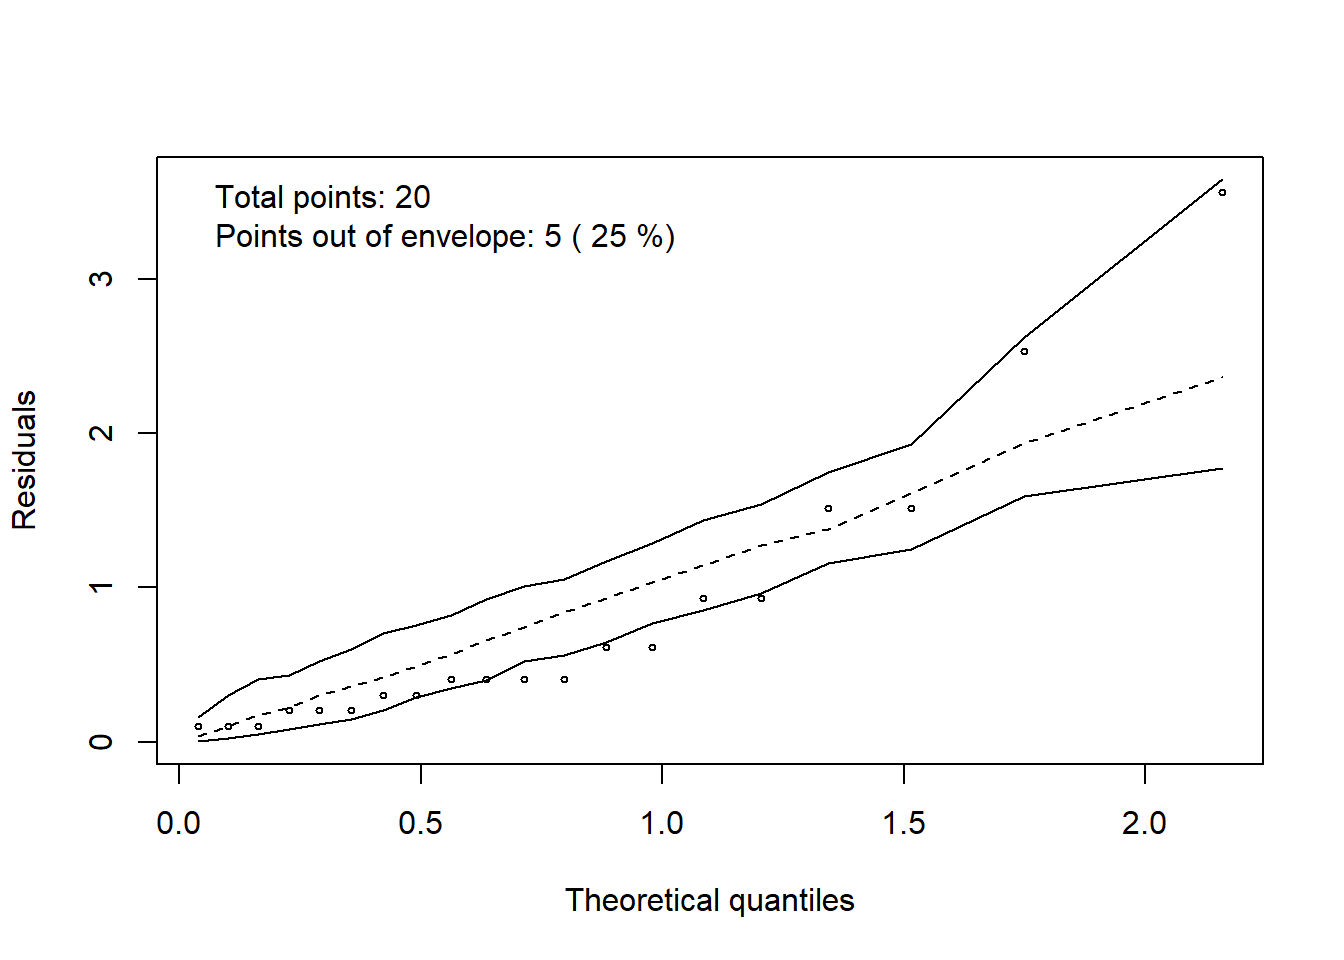
\includegraphics{aula12_GruposdeExp_files/figure-beamer/unnamed-chunk-12-1.pdf}
\end{frame}

\begin{frame}[fragile]{Análise conjunta: quadro auxiliar combinação
Local:Tratamento}
\protect\hypertarget{anuxe1lise-conjunta-quadro-auxiliar-combinauxe7uxe3o-localtratamento}{}
\begin{itemize}
\tightlist
\item
  Total
\end{itemize}

\begin{Shaded}
\begin{Highlighting}[]
\FunctionTok{with}\NormalTok{(dados,}
     \FunctionTok{tapply}\NormalTok{(altura, }\FunctionTok{list}\NormalTok{(Local, Trat), }
\NormalTok{            sum))}
\end{Highlighting}
\end{Shaded}

\begin{verbatim}
##      T1   T2   T3   T4    T5   T6
## L1 82.5 76.2 92.1 90.0  87.8 78.0
## L2 39.1 48.1 56.0 51.9  56.5 47.9
## L3 89.0 85.5 85.0 96.7 108.1 85.4
\end{verbatim}
\end{frame}

\begin{frame}[fragile]{Análise conjunta: quadro auxiliar combinação
Local:Tratamento}
\protect\hypertarget{anuxe1lise-conjunta-quadro-auxiliar-combinauxe7uxe3o-localtratamento-1}{}
\begin{itemize}
\tightlist
\item
  n
\end{itemize}

\begin{Shaded}
\begin{Highlighting}[]
\FunctionTok{with}\NormalTok{(dados,}
     \FunctionTok{tapply}\NormalTok{(altura, }\FunctionTok{list}\NormalTok{(Local, Trat), }
\NormalTok{            length))}
\end{Highlighting}
\end{Shaded}

\begin{verbatim}
##    T1 T2 T3 T4 T5 T6
## L1  4  4  4  4  4  4
## L2  4  4  4  4  4  4
## L3  4  4  4  4  4  4
\end{verbatim}
\end{frame}

\begin{frame}[fragile]{Análise conjunta: quadro auxiliar Local}
\protect\hypertarget{anuxe1lise-conjunta-quadro-auxiliar-local}{}
\begin{itemize}
\tightlist
\item
  Total
\end{itemize}

\begin{Shaded}
\begin{Highlighting}[]
\FunctionTok{with}\NormalTok{(dados,}
     \FunctionTok{tapply}\NormalTok{(altura, Local, }
\NormalTok{            sum))}
\end{Highlighting}
\end{Shaded}

\begin{verbatim}
##    L1    L2    L3 
## 506.6 299.5 549.7
\end{verbatim}

\begin{itemize}
\tightlist
\item
  n
\end{itemize}

\begin{Shaded}
\begin{Highlighting}[]
\FunctionTok{with}\NormalTok{(dados,}
     \FunctionTok{tapply}\NormalTok{(altura, Local, }
\NormalTok{            length))}
\end{Highlighting}
\end{Shaded}

\begin{verbatim}
## L1 L2 L3 
## 24 24 24
\end{verbatim}
\end{frame}

\begin{frame}[fragile]{Análise conjunta: quadro auxiliar Tratamentos}
\protect\hypertarget{anuxe1lise-conjunta-quadro-auxiliar-tratamentos}{}
\begin{itemize}
\tightlist
\item
  Total
\end{itemize}

\begin{Shaded}
\begin{Highlighting}[]
\FunctionTok{with}\NormalTok{(dados,}
     \FunctionTok{tapply}\NormalTok{(altura, Trat, }
\NormalTok{            sum))}
\end{Highlighting}
\end{Shaded}

\begin{verbatim}
##    T1    T2    T3    T4    T5    T6 
## 210.6 209.8 233.1 238.6 252.4 211.3
\end{verbatim}

\begin{itemize}
\tightlist
\item
  n
\end{itemize}

\begin{Shaded}
\begin{Highlighting}[]
\FunctionTok{with}\NormalTok{(dados,}
     \FunctionTok{tapply}\NormalTok{(altura, Trat, }
\NormalTok{            length))}
\end{Highlighting}
\end{Shaded}

\begin{verbatim}
## T1 T2 T3 T4 T5 T6 
## 12 12 12 12 12 12
\end{verbatim}
\end{frame}

\begin{frame}[fragile]{Razão entre os quadrados médios dos resíduos}
\protect\hypertarget{razuxe3o-entre-os-quadrados-muxe9dios-dos-resuxedduos}{}
\begin{Shaded}
\begin{Highlighting}[]
\NormalTok{(QMResiduo1}\OtherTok{\textless{}{-}} \FunctionTok{anova}\NormalTok{(mod.l1)}\SpecialCharTok{$}\StringTok{"Mean Sq"}\NormalTok{[}\DecValTok{3}\NormalTok{])}
\end{Highlighting}
\end{Shaded}

\begin{verbatim}
## [1] 3.783111
\end{verbatim}

\begin{Shaded}
\begin{Highlighting}[]
\NormalTok{(QMResiduo2}\OtherTok{\textless{}{-}} \FunctionTok{anova}\NormalTok{(mod.l2)}\SpecialCharTok{$}\StringTok{"Mean Sq"}\NormalTok{[}\DecValTok{3}\NormalTok{])}
\end{Highlighting}
\end{Shaded}

\begin{verbatim}
## [1] 3.755972
\end{verbatim}

\begin{Shaded}
\begin{Highlighting}[]
\NormalTok{(QMResiduo3}\OtherTok{\textless{}{-}} \FunctionTok{anova}\NormalTok{(mod.l3)}\SpecialCharTok{$}\StringTok{"Mean Sq"}\NormalTok{[}\DecValTok{3}\NormalTok{])}
\end{Highlighting}
\end{Shaded}

\begin{verbatim}
## [1] 1.435417
\end{verbatim}

\begin{Shaded}
\begin{Highlighting}[]
\NormalTok{(QMResiduo}\OtherTok{\textless{}{-}} \FunctionTok{c}\NormalTok{(QMResiduo1, QMResiduo2, QMResiduo3))}
\end{Highlighting}
\end{Shaded}

\begin{verbatim}
## [1] 3.783111 3.755972 1.435417
\end{verbatim}

\begin{Shaded}
\begin{Highlighting}[]
\NormalTok{(}\FunctionTok{max}\NormalTok{(QMResiduo)}\SpecialCharTok{/}\FunctionTok{min}\NormalTok{(QMResiduo))}
\end{Highlighting}
\end{Shaded}

\begin{verbatim}
## [1] 2.635549
\end{verbatim}
\end{frame}

\begin{frame}{ANOVA}
\protect\hypertarget{anova}{}
\(H_0:\)Não há efeito da interação Local\#Tratamento \emph{vs} \(H_1\):
Há efeito da interação Local\#Tratamento

\(H_0: \mu_{T1} = \mu_{T2} = \ldots = \mu_{T6}\) \emph{vs} \(H_1\): pelo
menos duas médias diferem entre si

\(H_0: \mu_{L1} = \mu_{L2} = \mu_{L3}\) \emph{vs} \(H_1\): pelo menos
duas médias diferem entre si
\end{frame}

\begin{frame}[fragile]{ANOVA}
\protect\hypertarget{anova-1}{}
\begin{Shaded}
\begin{Highlighting}[]
\NormalTok{mod.conj }\OtherTok{\textless{}{-}} \FunctionTok{aov}\NormalTok{(altura }\SpecialCharTok{\textasciitilde{}}\NormalTok{ Local}\SpecialCharTok{+}\NormalTok{Local}\SpecialCharTok{:}\NormalTok{Bloco}\SpecialCharTok{+}\NormalTok{Trat}\SpecialCharTok{+}\NormalTok{ Local}\SpecialCharTok{:}\NormalTok{Trat, }
                \AttributeTok{data=}\NormalTok{dados)}
\FunctionTok{anova}\NormalTok{(mod.conj)}
\end{Highlighting}
\end{Shaded}

\begin{verbatim}
## Analysis of Variance Table
## 
## Response: altura
##             Df  Sum Sq Mean Sq  F value  Pr(>F)    
## Local        2 1490.95  745.47 249.1969 < 2e-16 ***
## Trat         5  135.15   27.03   9.0357 5.3e-06 ***
## Local:Bloco  9   60.99    6.78   2.2652 0.03452 *  
## Local:Trat  10   76.57    7.66   2.5596 0.01530 *  
## Residuals   45  134.62    2.99                     
## ---
## Signif. codes:  0 '***' 0.001 '**' 0.01 '*' 0.05 '.' 0.1 ' ' 1
\end{verbatim}

Como o efeito da interação entre Locais e Tratamentos foi significativo
(\(\alpha = 0,05\)), vamos avaliar o efeito de Tratamentos dentro de
cada um dos Locais.
\end{frame}

\begin{frame}{Efeito de Tratamentos dentro de cada Local}
\protect\hypertarget{efeito-de-tratamentos-dentro-de-cada-local}{}
\(H_0: \mu_{L1T1} = \mu_{L1T2} = \ldots = \mu_{L1T6}\) \emph{vs}
\(H_1\): pelo menos duas médias diferem entre si

\(H_0: \mu_{L2T1} = \mu_{L2T2} = \ldots = \mu_{L2T6}\) \emph{vs}
\(H_1\): pelo menos duas médias diferem entre si

\(H_0: \mu_{L3T1} = \mu_{L3T2} = \ldots = \mu_{L3T6}\) \emph{vs}
\(H_1\): pelo menos duas médias diferem entre si
\end{frame}

\begin{frame}[fragile]{Efeito de Tratamentos dentro de cada Local}
\protect\hypertarget{efeito-de-tratamentos-dentro-de-cada-local-1}{}
\begin{Shaded}
\begin{Highlighting}[]
\NormalTok{mod.Tratd.Local}\OtherTok{\textless{}{-}} \FunctionTok{aov}\NormalTok{(altura }\SpecialCharTok{\textasciitilde{}}\NormalTok{ Local }\SpecialCharTok{+} 
\NormalTok{                        Local}\SpecialCharTok{:}\NormalTok{Bloco }\SpecialCharTok{+} 
\NormalTok{                        Local}\SpecialCharTok{:}\NormalTok{Trat, }
                      \AttributeTok{data=}\NormalTok{dados)}
\FunctionTok{anova}\NormalTok{(mod.Tratd.Local)}
\end{Highlighting}
\end{Shaded}

\begin{verbatim}
## Analysis of Variance Table
## 
## Response: altura
##             Df  Sum Sq Mean Sq  F value    Pr(>F)    
## Local        2 1490.95  745.47 249.1969 < 2.2e-16 ***
## Local:Bloco  9   60.99    6.78   2.2652   0.03452 *  
## Local:Trat  15  211.72   14.11   4.7183 2.526e-05 ***
## Residuals   45  134.62    2.99                       
## ---
## Signif. codes:  0 '***' 0.001 '**' 0.01 '*' 0.05 '.' 0.1 ' ' 1
\end{verbatim}
\end{frame}

\begin{frame}[fragile]{Efeito de Tratamentos dentro de cada Local}
\protect\hypertarget{efeito-de-tratamentos-dentro-de-cada-local-2}{}
Cabe salientar que a definição para os número de graus de liberdade irá
depender da ordem alfabética dos níveis dos fatores.

\begin{Shaded}
\begin{Highlighting}[]
\FunctionTok{summary}\NormalTok{(mod.Tratd.Local, }
        \AttributeTok{split=}\FunctionTok{list}\NormalTok{(}\StringTok{"Local:Trat"}\OtherTok{=}
                     \FunctionTok{list}\NormalTok{(}\AttributeTok{Td.L1 =} \FunctionTok{c}\NormalTok{(}\DecValTok{1}\NormalTok{,}\DecValTok{4}\NormalTok{,}\DecValTok{7}\NormalTok{,}\DecValTok{10}\NormalTok{,}\DecValTok{13}\NormalTok{),}
                          \AttributeTok{Td.L2 =} \FunctionTok{c}\NormalTok{(}\DecValTok{2}\NormalTok{,}\DecValTok{5}\NormalTok{,}\DecValTok{8}\NormalTok{,}\DecValTok{11}\NormalTok{,}\DecValTok{14}\NormalTok{), }
                          \AttributeTok{Td.L3 =} \FunctionTok{c}\NormalTok{(}\DecValTok{3}\NormalTok{,}\DecValTok{6}\NormalTok{,}\DecValTok{9}\NormalTok{,}\DecValTok{12}\NormalTok{,}\DecValTok{15}\NormalTok{))))}
\end{Highlighting}
\end{Shaded}
\end{frame}

\begin{frame}[fragile]{Efeito de Tratamentos dentro de cada Local}
\protect\hypertarget{efeito-de-tratamentos-dentro-de-cada-local-3}{}
\begin{verbatim}
##                     Df Sum Sq Mean Sq F value   Pr(>F)    
## Local                2 1490.9   745.5 249.197  < 2e-16 ***
## Local:Bloco          9   61.0     6.8   2.265  0.03452 *  
## Local:Trat          15  211.7    14.1   4.718 2.53e-05 ***
##   Local:Trat: Td.L1  5   53.5    10.7   3.577  0.00829 ** 
##   Local:Trat: Td.L2  5   52.2    10.4   3.487  0.00951 ** 
##   Local:Trat: Td.L3  5  106.1    21.2   7.091 5.80e-05 ***
## Residuals           45  134.6     3.0                     
## ---
## Signif. codes:  0 '***' 0.001 '**' 0.01 '*' 0.05 '.' 0.1 ' ' 1
\end{verbatim}

Há evidências para rejeitarmos as três hipóteses \(H_0\). Assim, pelo
menos duas médias de tratamentos diferem entre si em cada um dos três
locais (há efeito significativo de tratamentos dentro de cada um dos
locais).
\end{frame}

\begin{frame}[fragile]{Comparações múltiplas}
\protect\hypertarget{comparauxe7uxf5es-muxfaltiplas}{}
\begin{itemize}
\tightlist
\item
  Médias de Tratamentos dentro do Local 1 (Araraquara)
\end{itemize}

\begin{Shaded}
\begin{Highlighting}[]
\NormalTok{(Tukey.Tratd.L1 }\OtherTok{\textless{}{-}} \FunctionTok{with}\NormalTok{(}\FunctionTok{subset}\NormalTok{(dados, Local }\SpecialCharTok{==} \StringTok{"L1"}\NormalTok{),}
                        \FunctionTok{HSD.test}\NormalTok{(altura, }
\NormalTok{                                 Trat,}
                                 \DecValTok{45}\NormalTok{,}
                                 \FloatTok{3.0}\NormalTok{)))}
\end{Highlighting}
\end{Shaded}
\end{frame}

\begin{frame}[fragile]{Comparações múltiplas}
\protect\hypertarget{comparauxe7uxf5es-muxfaltiplas-1}{}
\begin{itemize}
\tightlist
\item
  Médias de Tratamentos dentro do Local 1 (Araraquara)
\end{itemize}

\begin{verbatim}
## $statistics
##   MSerror Df     Mean       CV      MSD
##         3 45 21.10833 8.205531 3.644814
## 
## $parameters
##    test name.t ntr StudentizedRange alpha
##   Tukey   Trat   6         4.208669  0.05
## 
## $means
##    altura      std r        se  Min  Max    Q25   Q50    Q75
## T1 20.625 1.978846 4 0.8660254 19.1 23.5 19.475 19.95 21.100
## T2 19.050 2.074448 4 0.8660254 16.7 21.7 18.050 18.90 19.900
## T3 23.025 1.950000 4 0.8660254 20.8 24.9 21.700 23.20 24.525
## T4 22.500 1.856520 4 0.8660254 20.8 24.9 21.175 22.15 23.475
## T5 21.950 0.341565 4 0.8660254 21.5 22.3 21.800 22.00 22.150
## T6 19.500 1.838478 4 0.8660254 17.7 22.0 18.450 19.15 20.200
## 
## $comparison
## NULL
## 
## $groups
##    altura groups
## T3 23.025      a
## T4 22.500     ab
## T5 21.950     ab
## T1 20.625     ab
## T6 19.500     ab
## T2 19.050      b
## 
## attr(,"class")
## [1] "group"
\end{verbatim}
\end{frame}

\begin{frame}[fragile]{Comparações múltiplas}
\protect\hypertarget{comparauxe7uxf5es-muxfaltiplas-2}{}
\begin{itemize}
\tightlist
\item
  Médias de Tratamentos dentro do Local 1 (Araraquara)
\end{itemize}

\begin{verbatim}
##    altura groups
## T3 23.025      a
## T4 22.500     ab
## T5 21.950     ab
## T1 20.625     ab
## T6 19.500     ab
## T2 19.050      b
\end{verbatim}
\end{frame}

\begin{frame}[fragile]{Comparações múltiplas}
\protect\hypertarget{comparauxe7uxf5es-muxfaltiplas-3}{}
\begin{itemize}
\tightlist
\item
  Médias de Tratamentos dentro do Local 2 (Bento Quirino)
\end{itemize}

\begin{Shaded}
\begin{Highlighting}[]
\NormalTok{(Tukey.Tratd.L2 }\OtherTok{\textless{}{-}} \FunctionTok{with}\NormalTok{(}\FunctionTok{subset}\NormalTok{(dados, Local }\SpecialCharTok{==} \StringTok{"L2"}\NormalTok{),}
                        \FunctionTok{HSD.test}\NormalTok{(altura, }
\NormalTok{                                 Trat,}
                                 \DecValTok{45}\NormalTok{,}
                                 \FloatTok{3.0}\NormalTok{)))}
\end{Highlighting}
\end{Shaded}
\end{frame}

\begin{frame}[fragile]{Comparações múltiplas}
\protect\hypertarget{comparauxe7uxf5es-muxfaltiplas-4}{}
\begin{itemize}
\tightlist
\item
  Médias de Tratamentos dentro do Local 2 (Bento Quirino)
\end{itemize}

\begin{verbatim}
## $statistics
##   MSerror Df     Mean       CV      MSD
##         3 45 12.47917 13.87954 3.644814
## 
## $parameters
##    test name.t ntr StudentizedRange alpha
##   Tukey   Trat   6         4.208669  0.05
## 
## $means
##    altura      std r        se  Min  Max    Q25   Q50    Q75
## T1  9.775 1.543535 4 0.8660254  8.1 11.7  8.850  9.65 10.575
## T2 12.025 2.729316 4 0.8660254 10.3 16.1 10.675 10.85 12.200
## T3 14.000 2.801190 4 0.8660254 11.0 17.7 12.575 13.65 15.075
## T4 12.975 1.352467 4 0.8660254 11.2 14.4 12.400 13.15 13.725
## T5 14.125 4.280479 4 0.8660254 11.3 20.5 11.975 12.35 14.500
## T6 11.975 1.007886 4 0.8660254 10.6 13.0 11.650 12.15 12.475
## 
## $comparison
## NULL
## 
## $groups
##    altura groups
## T5 14.125      a
## T3 14.000      a
## T4 12.975     ab
## T2 12.025     ab
## T6 11.975     ab
## T1  9.775      b
## 
## attr(,"class")
## [1] "group"
\end{verbatim}
\end{frame}

\begin{frame}[fragile]{Comparações múltiplas}
\protect\hypertarget{comparauxe7uxf5es-muxfaltiplas-5}{}
\begin{itemize}
\tightlist
\item
  Médias de Tratamentos dentro do Local 2 (Bento Quirino)
\end{itemize}

\begin{verbatim}
##    altura groups
## T5 14.125      a
## T3 14.000      a
## T4 12.975     ab
## T2 12.025     ab
## T6 11.975     ab
## T1  9.775      b
\end{verbatim}
\end{frame}

\begin{frame}[fragile]{Comparações múltiplas}
\protect\hypertarget{comparauxe7uxf5es-muxfaltiplas-6}{}
\begin{itemize}
\tightlist
\item
  Médias de Tratamentos dentro do Local 3 (Mogi-Guaçu)
\end{itemize}

\begin{Shaded}
\begin{Highlighting}[]
\NormalTok{(Tukey.Tratd.L3 }\OtherTok{\textless{}{-}} \FunctionTok{with}\NormalTok{(}\FunctionTok{subset}\NormalTok{(dados, Local }\SpecialCharTok{==} \StringTok{"L3"}\NormalTok{),}
                        \FunctionTok{HSD.test}\NormalTok{(altura, }
\NormalTok{                                 Trat,}
                                 \DecValTok{45}\NormalTok{,}
                                 \FloatTok{3.0}\NormalTok{)))}
\end{Highlighting}
\end{Shaded}
\end{frame}

\begin{frame}[fragile]{Comparações múltiplas}
\protect\hypertarget{comparauxe7uxf5es-muxfaltiplas-7}{}
\begin{itemize}
\tightlist
\item
  Médias de Tratamentos dentro do Local 3 (Mogi-Guaçu)
\end{itemize}

\begin{verbatim}
## $statistics
##   MSerror Df     Mean       CV      MSD
##         3 45 22.90417 7.562165 3.644814
## 
## $parameters
##    test name.t ntr StudentizedRange alpha
##   Tukey   Trat   6         4.208669  0.05
## 
## $means
##    altura       std r        se  Min  Max    Q25   Q50    Q75
## T1 22.250 0.6855655 4 0.8660254 21.4 22.9 21.850 22.35 22.750
## T2 21.375 0.8732125 4 0.8660254 20.7 22.6 20.775 21.10 21.700
## T3 21.250 1.3178265 4 0.8660254 19.4 22.5 20.900 21.55 21.900
## T4 24.175 0.8500000 4 0.8660254 23.3 25.0 23.525 24.20 24.850
## T5 27.025 0.7762087 4 0.8660254 26.4 28.0 26.400 26.85 27.475
## T6 21.350 1.7597348 4 0.8660254 19.4 23.5 20.300 21.25 22.300
## 
## $comparison
## NULL
## 
## $groups
##    altura groups
## T5 27.025      a
## T4 24.175     ab
## T1 22.250      b
## T2 21.375      b
## T6 21.350      b
## T3 21.250      b
## 
## attr(,"class")
## [1] "group"
\end{verbatim}
\end{frame}

\begin{frame}[fragile]{Comparações múltiplas}
\protect\hypertarget{comparauxe7uxf5es-muxfaltiplas-8}{}
\begin{itemize}
\tightlist
\item
  Médias de Tratamentos dentro do Local 3 (Mogi-Guaçu)
\end{itemize}

\begin{verbatim}
##    altura groups
## T5 27.025      a
## T4 24.175     ab
## T1 22.250      b
## T2 21.375      b
## T6 21.350      b
## T3 21.250      b
\end{verbatim}
\end{frame}

\begin{frame}[fragile]{Gráfico}
\protect\hypertarget{gruxe1fico}{}
\begin{Shaded}
\begin{Highlighting}[]
\NormalTok{Tukey.Tratd.L1}\SpecialCharTok{$}\NormalTok{groups}\SpecialCharTok{$}\NormalTok{Trat }\OtherTok{\textless{}{-}} 
  \FunctionTok{rownames}\NormalTok{(Tukey.Tratd.L1}\SpecialCharTok{$}\NormalTok{groups)}
\NormalTok{Tukey.Tratd.L1}\SpecialCharTok{$}\NormalTok{groups}\SpecialCharTok{$}\NormalTok{Local }\OtherTok{\textless{}{-}} \StringTok{"L1"}
\NormalTok{Tukey.Tratd.L2}\SpecialCharTok{$}\NormalTok{groups}\SpecialCharTok{$}\NormalTok{Trat }\OtherTok{\textless{}{-}} 
  \FunctionTok{rownames}\NormalTok{(Tukey.Tratd.L2}\SpecialCharTok{$}\NormalTok{groups)}
\NormalTok{Tukey.Tratd.L2}\SpecialCharTok{$}\NormalTok{groups}\SpecialCharTok{$}\NormalTok{Local }\OtherTok{\textless{}{-}} \StringTok{"L2"}
\NormalTok{Tukey.Tratd.L3}\SpecialCharTok{$}\NormalTok{groups}\SpecialCharTok{$}\NormalTok{Trat }\OtherTok{\textless{}{-}} 
  \FunctionTok{rownames}\NormalTok{(Tukey.Tratd.L3}\SpecialCharTok{$}\NormalTok{groups)}
\NormalTok{Tukey.Tratd.L3}\SpecialCharTok{$}\NormalTok{groups}\SpecialCharTok{$}\NormalTok{Local }\OtherTok{\textless{}{-}} \StringTok{"L3"}

\NormalTok{Tukey.Trat }\OtherTok{\textless{}{-}} \FunctionTok{data.frame}\NormalTok{(}\FunctionTok{rbind}\NormalTok{(}
\NormalTok{  Tukey.Tratd.L1}\SpecialCharTok{$}\NormalTok{groups,}
\NormalTok{  Tukey.Tratd.L2}\SpecialCharTok{$}\NormalTok{groups,}
\NormalTok{  Tukey.Tratd.L3}\SpecialCharTok{$}\NormalTok{groups}
\NormalTok{))}
\end{Highlighting}
\end{Shaded}
\end{frame}

\begin{frame}[fragile]{Gráfico}
\protect\hypertarget{gruxe1fico-1}{}
\begin{Shaded}
\begin{Highlighting}[]
\FunctionTok{ggplot}\NormalTok{(Tukey.Trat,}
       \FunctionTok{aes}\NormalTok{(}\AttributeTok{x =}\NormalTok{ Trat,}
           \AttributeTok{y =}\NormalTok{ altura,}
           \AttributeTok{label =}\NormalTok{ groups,}
           \AttributeTok{fill =}\NormalTok{ Trat)) }\SpecialCharTok{+}
  \FunctionTok{geom\_bar}\NormalTok{(}\AttributeTok{stat =} \StringTok{"identity"}\NormalTok{) }\SpecialCharTok{+}
  \FunctionTok{facet\_grid}\NormalTok{(}\SpecialCharTok{\textasciitilde{}}\NormalTok{ Local) }\SpecialCharTok{+}
  \FunctionTok{geom\_text}\NormalTok{(}\FunctionTok{aes}\NormalTok{(}\AttributeTok{x =}\NormalTok{ Trat,}
                \AttributeTok{y =}\NormalTok{ altura }\SpecialCharTok{+} \DecValTok{1}\NormalTok{)) }\SpecialCharTok{+}
  \FunctionTok{xlab}\NormalTok{(}\StringTok{"Tratamentos"}\NormalTok{) }\SpecialCharTok{+}
  \FunctionTok{ylab}\NormalTok{(}\StringTok{"altura (m)"}\NormalTok{)}
\end{Highlighting}
\end{Shaded}
\end{frame}

\begin{frame}{Gráfico}
\protect\hypertarget{gruxe1fico-2}{}
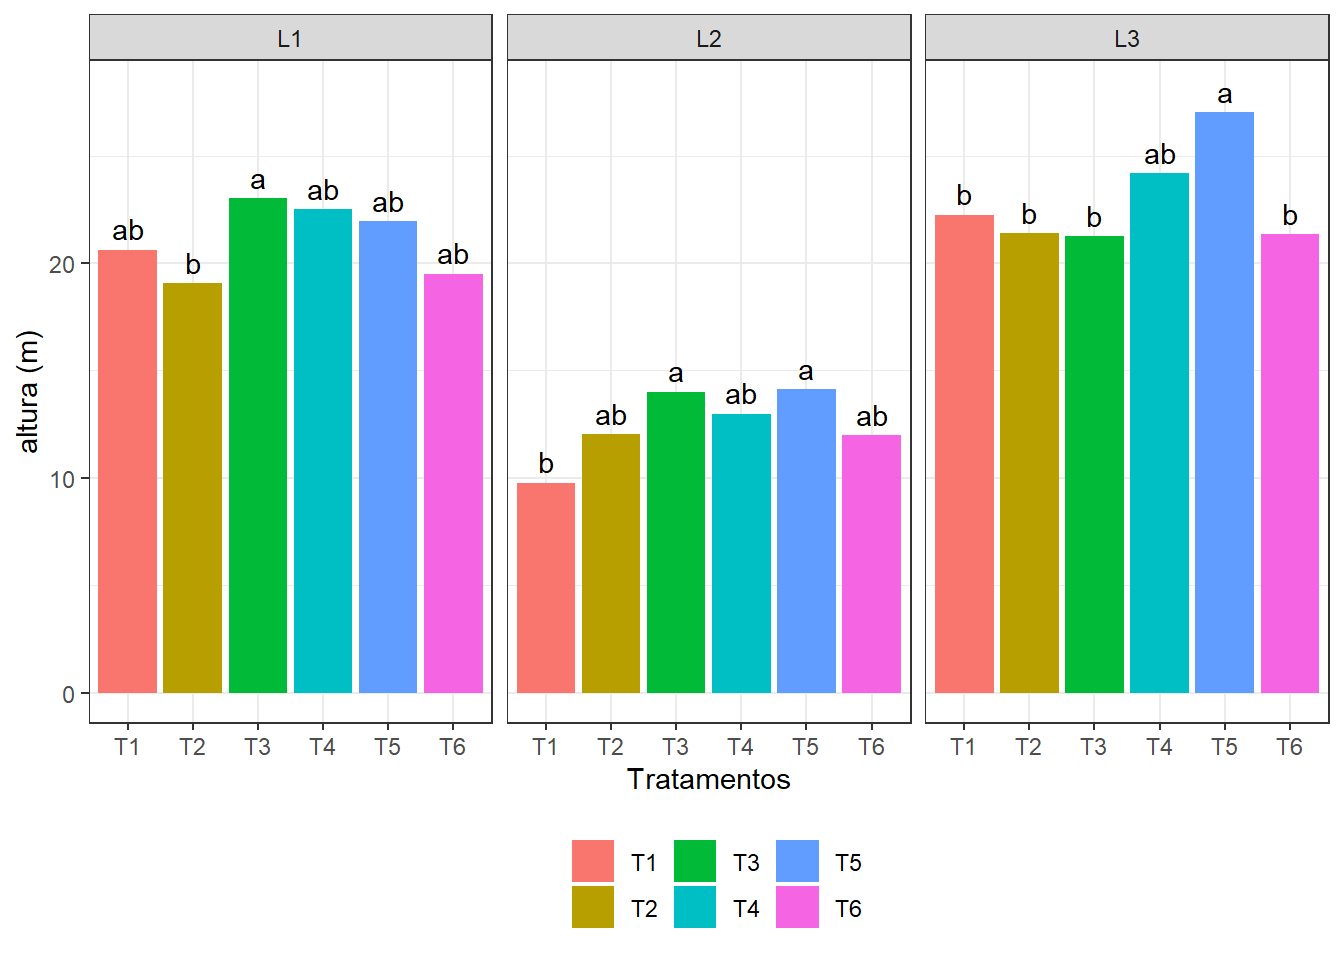
\includegraphics{aula12_GruposdeExp_files/figure-beamer/unnamed-chunk-35-1.pdf}
\end{frame}

\end{document}
